\chapter{Experimental Methodology}
\label{methodology}

\section{Anechoic Chamber}
All experiments were conducted at the GDTL within the Aerospace Research Center at the Ohio State University. 
Compressed, dried, and filtered air is supplied to the facility from two cylindrical storage tanks with a total capacity of 43 m$^{3}$ and maximum storage pressure of 16 MPa.
The air may be routed through a storage heater (not used in this study), which allows the jet to operate with a stagnation temperature up to 500 C, before expanding through a nozzle and exhausting horizontally into an anechoic chamber. 
Opposite the nozzle, a collector accumulates the jet and entrained air and exhausts to the outdoors. 
A schematic of the anechoic chamber can be seen in [INSERT FIGURE]. 
The dimensions of the chamber are 6.20 m wide by 5.59 m long and 3.36 m tall, with internal wedge-tip to wedge-tip dimensions of 5.14 m by 4.48 m and 2.53 m, respectively. 
The design of the chamber produces a cutoff frequency of 160 Hz, below the frequencies of interest for this study. 
A more detailed description of the GDTL anechoic chamber properties and validation has been given by [Hahn?].
\begin{figure}
	\centering
	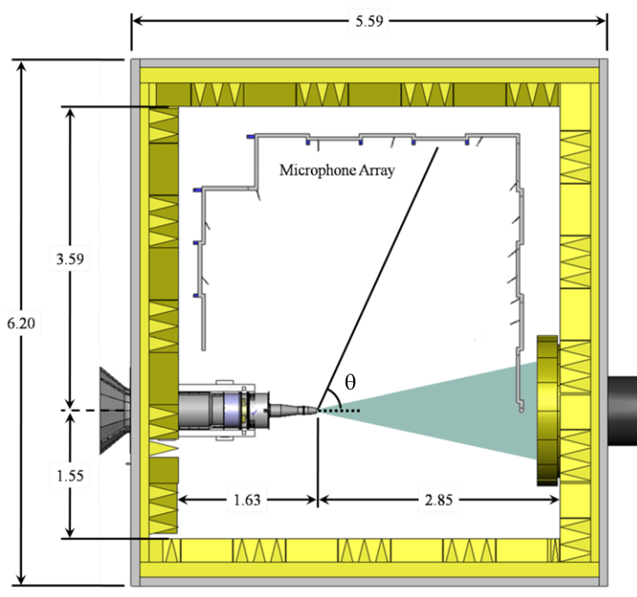
\includegraphics{Figures/Chamber_Schematic.png}
	\caption{Top-down view of anechoic chamber and free jet facility at GDTL; dimensions are in meters.} 
	\label{fig:chamber}
\end{figure}

For this study a converging, axisymmetric nozzle with exit diameter D of 25.4 mm was used. 
The internal contour of the nozzle was designed using a fifth order polynomial. 
The nozzle utilized a thick-lipped design in order to simplify the mounts for the LAFPA extension, which housed the eight actuators used in this study. 
For the experiments reported in this paper, the jet was operated at a Mach number ($M_j$) of 0.90, and with a total temperature ratio of approximately unity. 
The Reynolds number based on the jet exit diameter was $6.2\times〖10〗^5$; previous investigations using hot-wire anemometry have indicated that the initial shear layer is turbulent for this operating condition with momentum thickness ~0.09 mm and boundary layer thickness ~1 mm [Kearney?].

\section{Data Acquisition}
\subsection{Near- and Far-field Pressure}
Near-field and far-field pressure measurements were acquired simultaneously, using Brüel \& Kjær ¼ inch 4939 microphones. 
The signal from each microphone is band-pass filtered from 20 Hz to 100 kHz using a Brüel \& Kjær Nexus 2690 conditioning amplifier, and recorded using National Instruments PXI-6133 A/D boards and LabVIEW software. 
The microphones are calibrated using a Brüel \& Kjaer 114 dB, 1 kHz sine wave generator (model \# ???). 
The frequency response of the microphones is flat up to roughly 80 kHz, with the protective grid covers removed. 

\subsection{Particle Image Velocimetry}
The instantaneous velocity was acquired using streamwise, two-component particle image velocimetry (PIV). 
A Spectra Physics, double-pulsed Nd:YAG laser (model PIV-400) was used as the illumination source. 
Due to facility requirements, the laser was located on a vibrationally-damped table outside the anechoic chamber and the laser beam was routed into the chamber using an overhead port; this resulted in a beampath of $\sim$10~m. 
The laser sheet was formed using two cylindrical and one spherical lens; one of the cylindrical lenses was mounted to a rotational stage in order to ensure that the final laser sheet was normal to the jet exit (i.e. the laser sheet was streamwise to the jet).
Alignment of the separate laser heads was initially performed using burn paper; final alignment was performed by seeding a low-velocity flow and visually checking that the same particles were captured in both frames.

The jet core was seeded using Di-Ethyl-Hexyl-Sebacat (DEHS); the oil was atomized using a LaVision Aerosol generator and injected upstream of the turbulence screens in the stagnation chamber in order to produce a uniform seed particle density.
As the jet entrains a significant amount of the surrounding ambient fluid as it evolves downstream, the coflow around the jet must also be seeded in order to accurately measure the outer shear layer velocity.
For this, a TSI 6-jet atomizer (model 9306A) and olive oil was used; injection occurred into a plenum which surrounded the core stagnation chamber.
To ensure consistent seeding, this coflow was driven using a small blower (Model number???) and a series of high-pressure ejectors. 
As a result, for the PIV data acquisitions, the jet core was surrounded by a $\sim$5~m/s coflow. 
Per the manufacturer's specfications, both atomizers provided nominally sub-micron seed particles.

Image groups were acquired using two LaVision Imager Pro SX 5M cameras.
The cameras had 12-bit resolution and 2560$\times$2180 pixels.
The combination of the PIV-400 laser and the Imager Pro SX cameras resulted in a maximum acquisition rate for the image groups of 5~Hz.
Nikon Nikkor 105~mm f/1.8 lenses were used, and 532~nm bandpass filters were mounted on the lenses (what is the maker for the filters?!?!).
The cameras were positioned such that they were nominally normal to the image plane, negating the need for scheimpflug mounts.
This was done as having high spatial resolution and field of view were deemed to be more important than having full, three-component velocity vectors.
The cameras were aligned such that there was roughly a 10\% overlap between the two images.
This setup is generally designated as ``side-to-side'' in order to differentiate it from stereoscopic PIV.
The cameras were calibrated simultaneously using a LaVision calibration plate (type 31). 
Hardware background subtraction was used in order to reduce the effect of reflections off of the nozzle extension and near-field microphone array.

Instantaneous velocity vectors were computed using LaVision's DaVis software.
Multipass, FFT-based cross-correlations were used, with decreasing window size (64$\times$64 for the initial pass, and 32$\times$32 for the final two passes).
A 75\% overlap was used for all passes.
The velocity fields were post-processed to remove spurious vectors, which were iteratively replaced if secondary correlation peaks were found, before the downstream and upstream images were combined.
No interpolation, smoothing, or denoising was performed in post-processing.

\section{Localized Arc-Filament Plasma Actuators}